\documentclass[14pt,a4paper]{article}
\usepackage[utf8]{inputenc}
\usepackage[T1]{fontenc}
\usepackage{amsmath}
\usepackage{amsfonts}
\usepackage{amssymb}
\usepackage{graphicx}
\usepackage{hyperref}
\usepackage[style=authoryear,backend=biber]{biblatex}
\DeclareDelimFormat{postnotedelim}{\addcomma\space}
\usepackage{csquotes}
\usepackage[margin=3.5cm]{geometry}
\usepackage{titlesec}
\usepackage{appendix}
\usepackage{booktabs}
\usepackage{longtable}
\usepackage{fancyhdr}
\usepackage{xurl}

\addbibresource{references.bib}

\titleformat{\section}
  {\normalfont\Large\bfseries}{\thesection}{1em}{}
\titleformat{\subsection}
  {\normalfont\large\bfseries}{\thesubsection}{1em}{}

\title{Goal-Oriented Requirements Engineering (i*)}
\author{Socio-Technical Evaluation of the Car Repair Shop with i* Modelling}
\date{}

\renewcommand{\labelitemi}{-}

\pagestyle{fancy}
\fancyhf{}
\renewcommand{\headrulewidth}{0.4pt}
\renewcommand{\footrulewidth}{0.4pt}
\fancyhead[L]{UFCFAF-30-3 | Development of Information Systems Projects}
\fancyhead[R]{Page \thepage}
\fancyfoot[C]{\thepage}

\begin{document}

\maketitle

\hrule

\vspace{3em}

UFCFAF-30-3 | Development of Information Systems Projects

Word Count: 965

\vspace{3em}
\hrule

\vspace{2em}

\textbf{\Large{Abstract}}
\vspace{1em}

Goal-Oriented Requirements Engineering (GORE) positions information systems within organisational and interpersonal contexts, addressing limitations of traditional requirement approaches. This paper dissects our application of i* modelling for the Car Repair Shop case study, focussing specifically on the implementation of socio-technical dimensions to the model and the basis of theory behind our decision-making in doing so. Through systematic analysis of strategic dependencies and the extensive provision of rationales among the given actors, our model demonstrates how key quality attributes and trust relationships fundamentally shape system requirements. The paper highlights the capture of intentions, dependencies, and quality constraints in the socio-technical model that conventional approaches to requirement engineering frequently overlook.

\vspace{3em}
\hrule

\thispagestyle{empty}

\tableofcontents
\pagenumbering{roman}

\newpage

\pagenumbering{arabic}

\section{Introduction}

Our i* model  applies concepts from \textcite[p. 127]{Yu2011}, capturing "intentional characteristics of social actors, their interrelationships, concerns, vulnerabilities, and opportunities." Unlike standard UML diagrams focussing on processes, our model reveals motivations and quality constraints underlying system behaviour, demonstrating what \textcite[p. 342]{Dalpiaz2016} identify as "strategic dimensions of socio-technical systems."

Our implementation identifies four actor with distinct goals, tasks, resources, and quality attributes that define the business ecosystem.

\begin{figure}[ht]
  \hspace{-6.5em}
    \begin{minipage}[t]{1.3\textwidth}
        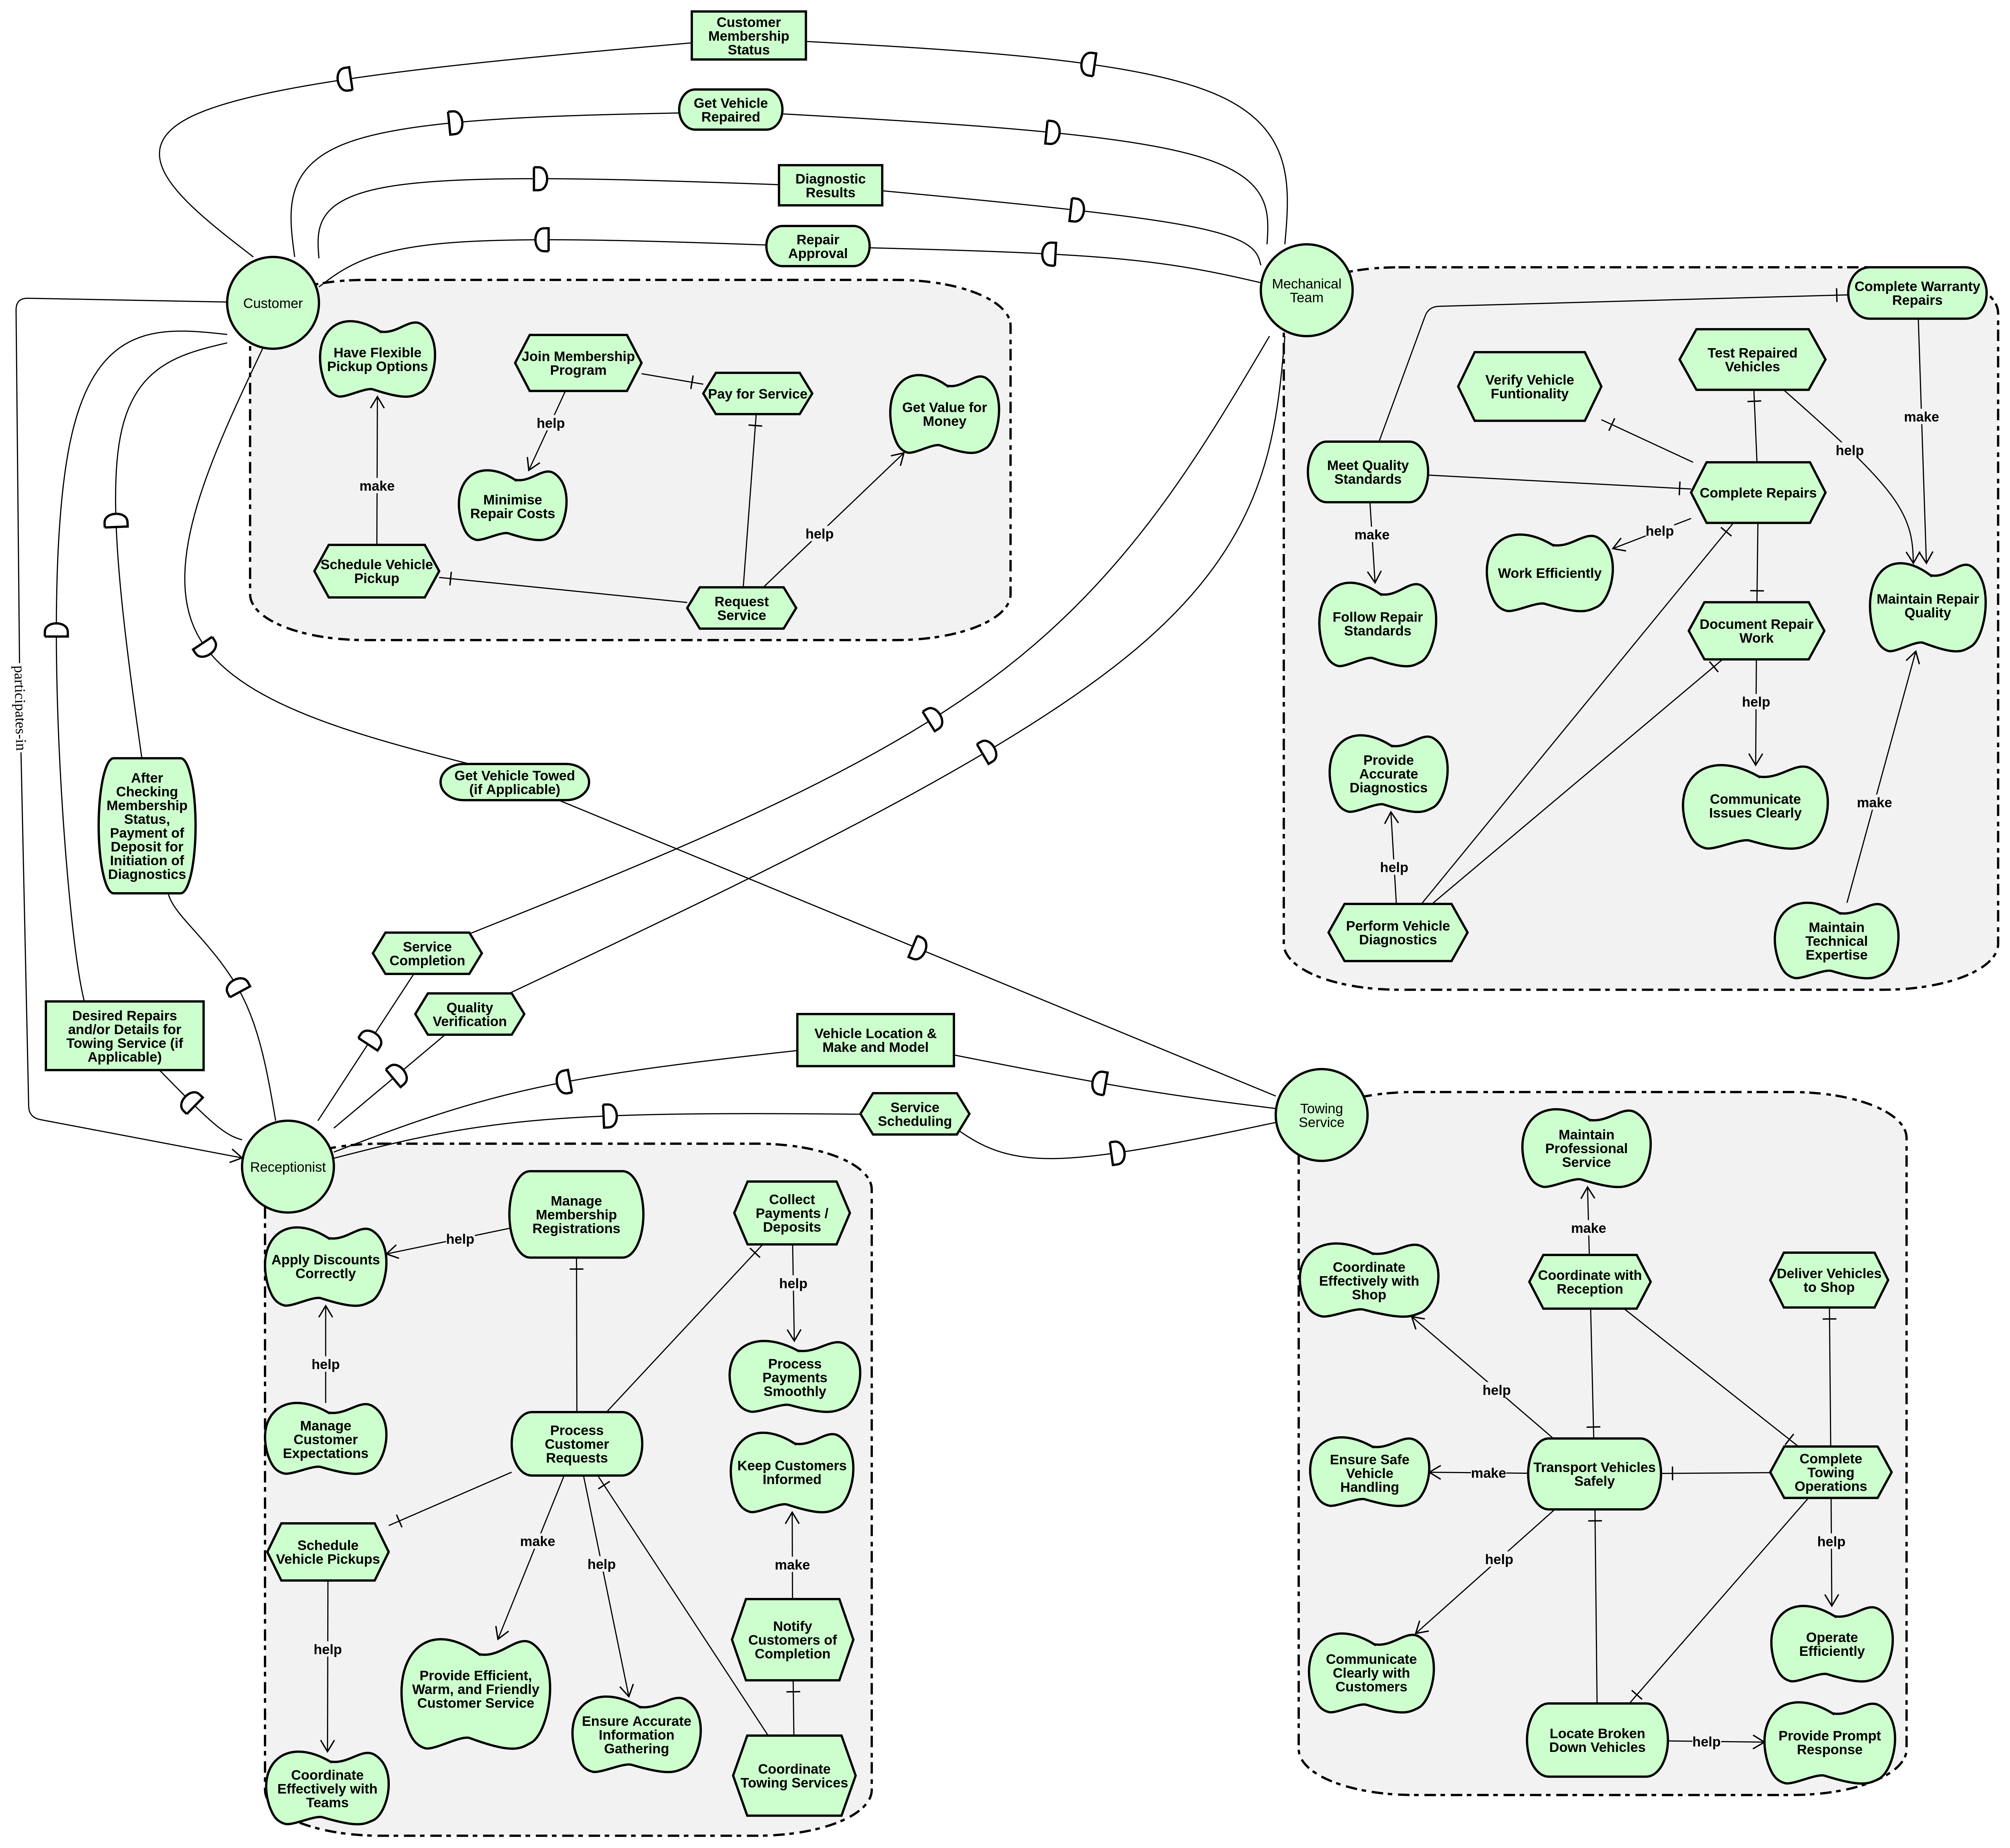
\includegraphics[width=\linewidth]{istar.png}
        \caption{i*, Goal-Oriented Requirements Model}
    \end{minipage}
\end{figure}

\section{Modelling Implementation}

Our implementation follows the iStar 2.0 specification \parencite[p. 344]{Dalpiaz2016}, constructing a comprehensive actor model of automotive repair operations. The model addresses what \textcite[p. 87]{Sommerville2016} identifies as "the fundamental disconnect between technical specification and human motivation" through explicit representation of:

\begin{itemize}
    \item \textbf{Goals}: "Get Vehicle Repaired," "Transport Vehicles Safely," "Meet Quality Standards"
    \item \textbf{Tasks}: "Perform Vehicle Diagnostics," "Schedule Vehicle Pickup," "Coordinate Towing Services"
    \item \textbf{Resources}: "Vehicle Location \& Make and Model," "Diagnostic Results," "Customer Membership Status"
    \item \textbf{Quality Attributes}: "Minimise Repair Costs," "Provide Efficient, Warm, and Friendly Customer Service"
\end{itemize}

The model reveals what \textcite[p. 78]{Horkoff2019} term "critical dependency vulnerabilities" (such as the Customer's depending on the Mechanic for Diagnostic Results) that directly influence system-wide requirements. Our implementation particularly emphasises the membership programme's dual role as a financial incentive but also a B2C relationship management mechanism, an exemplary and consummate instance of what \textcite[p. 177]{Estrada2020} identify as "multi-dimensional strategic instruments" that we might endeavour significantly to shape the system's design around.

Strategic analysis of dependencies reveals critical interaction points requiring specific support, particularly the Customer-Receptionist relationship where payment processing, service explanation, and coordination of the repair converge. The model explicitly visualises how the Receptionist's task "Notify Customers of Completion" contributes to the quality attribute "Keep Customers Informed" - establishing a direct requirement and capability for notification across the system.

\section{Socio-Technical Insights}

Our i* model reveals three critical socio-technical dimensions for consideration with respect to system requirements:

\begin{enumerate}
  \item \textbf{Trust Dependencies}: The Customer's reliance on repair quality and the Mechanic's dependency on approval create what \textcite[p. 73]{Rifaut2020} term "critical trust points." Our model explicitly captures this through dependencies "Repair Approval" and "Diagnostic Results," highlighting information asymmetry that the system must address. The task of "Document[ing] Repair Work" directly contributes to and facilitates "Communicat[ing] Issues Clearly," establishing requirements for transparency alongside record-keeping mechanisms.

    \item \textbf{Quality-Efficiency Tensions}: Our model reveals inherent conflicts between competing quality attributes (what \textcite[p. 41]{Lezcano2022} identify as "characteristic socio-technical conflicts"). The Mechanic balances "Work[ing] Efficiently" and "Maintain[ing] Repair Quality," creating trade-offs that system design and ultimately the actors themselves must accommodate. This tension manifests particularly in task relationships where thorough diagnosis competes with operational efficiency, and by extension upholding stellar customer service standards.

    \item \textbf{Coordination Requirements}: The model exposes critical coordination needs between actors through dependencies like "Service Completion" and "Quality Verification" flowing from Receptionist to Mechanic. This creates what \textcite[p. 132]{Samavi2019} describe as "boundary-spanning information requirements" necessitating system features that facilitate cross-functional workflow management.
\end{enumerate}

The membership programme emerges as a strategic mechanism with wide-ranging, deeply resounding effects on the entire system. The Customer's task "Join Membership Program" contributes to "Minimise Repair Costs," while creating coordination requirements between actors. The Receptionist's goal "Manage Membership Registrations" directly influences the quality attribute "Apply Discounts Correctly" - establishing specific system capabilities for membership verification and privilege application.

\section{Strategic Implications}

Our i* model yields significant implications for system requirements, explicitly revealing socio-technical factors requiring specific support:

First, the customer service quality attribute to "Provide Efficient, Warm, and Friendly Customer Service" demonstrates what \textcite[p. 304]{Carvallo2006} identify as "nontechnical quality factors [sharing] some fundamental properties [with technical ones]." This quality attribute suggests for system-wide enabling of personable interactions and good service for relationship management, as opposed to cold transactional processing.

Second, the actor boundary between Receptionist and Mechanic creates what \textcite[p. 48]{Gorton2017} term "critical information translation requirements" necessitating workflow coordination features. Dependencies "Service Completion" and "Quality Verification" establish explicit requirements for status tracking and quality assurance protocols.

Third, the Towing Service integration creates time-sensitive coordination requirements captured through dependencies "Vehicle Location \& Make and Model" and "Service Scheduling." These dependencies establish system requirements for informational and appointment management-features that might otherwise remain implicit using traditional approaches.

\section{Conclusion}

Our i* diagram demonstrates that services such as the Car Repair Shop, which one might at first glance suspect to be uncomplicated, can represent complex socio-technical ecosystems where strategic relationships fundamentally influence operational effectiveness, capabilities, and needs. The model reveals that successful system implementation requires diligent attention to both explicit technical workflows and implicit social structures, confirming the observation of \textcite[p. 47]{Lezcano2022} that "systems development success depends not merely on functional correctness but on alignment with organisational motivations."

Through systematic modelling of strategic dependencies followed by stategic dependency rationales, our implementation exposes quality attributes, trust dynamics, key business process relationships, and coordination of all the above requirements that many conventional approaches to requirements engineering have historically failed to identify. Particularly significant is the identification of competing quality constraints - efficiency versus thoroughness, cost versus quality - that establish critical trade-off points requiring careful system design. After all, a constraint is merely a requirement by another name.

The membership programme emerges as a strategic mechanism influencing multiple actors, while the emphasis on warm, friendly, and reliable service alongside a high level of technical competence presents aptly the dualistic natural balance inherent of business service system requirements. By explicitly modelling these elements, our i* implementation demonstrates how comprehensive socio-technical analysis significantly enhances requirements elicitation for complex service-oriented systems, and aids the progression of our development into Business Process Management Notation and automation.

\newpage

\printbibliography

\end{document}
